\documentclass[a4paper,12pt]{article}
\usepackage[utf8]{inputenc}   %para los acentos
\usepackage[left=25mm,right=25mm,top=25mm,bottom=25mm]{geometry}
% \usepackage[left=25mm,right=25mm,top=15mm,bottom=25mm,includefoot,includehead,headheight=1pt]{geometry}
\usepackage{bold-extra}
\usepackage{amsmath} %para los \text dentro de $ $
\usepackage{graphicx}
\hyphenation{pro-ble-ma}

\begin{document}

% \centering \large \textsc{\textbf{Introducción a la Magnetohidrodinámica}} \\
\begin{center}
{\large\textbf{Magneto-hydrodynamical simulations of sub-parsec circumbinary discs
}} \\

\end{center}

\bigskip

\section{Initial conditions}

In this section we describe the initial conditions.

We model our system using a modified version of the
smoothed particle hydrodynamics (SPH) code gadget-3,
which is an improved version of the public code gadget-2
(Springel 2005).
We are simulating the same system described in Cuadra
et al. (2009), with the binary with initially mass ratio of
$q = 1/3$ and with circular orbit. The initial mass of the disc
is $M_\text{d} = 0.2M_{\text{bin}}$. The initial conditions are set such as the
gas is located from $r_{\text{in}} = 0.2a$ to $r_{\text{out}} = 0.5a$, where $a$ is the
binary semi-major axis (Fig. 1). However, we want to avoid spurious growth of the magnetic field due to steep gradients and
the violent initial evolution of the disc, therefore we use as
initial condition a system that is already in a quasi-steady
equilibrium. We start with a system that is already evolves
for 500 dynamical times ($250/\pi$ orbits), as the one shown in
Fig. 2.
\begin{figure}[!ht]
 \begin{center}
 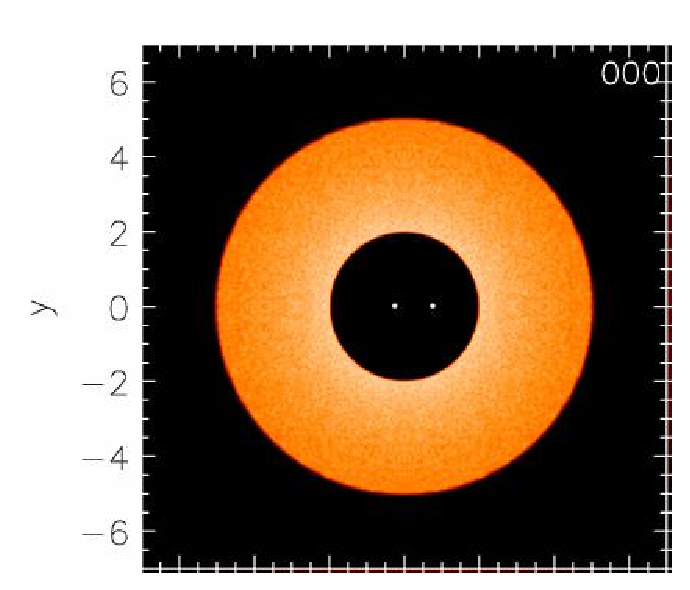
\includegraphics[width=0.4\textwidth]{figs/fig1.eps}
  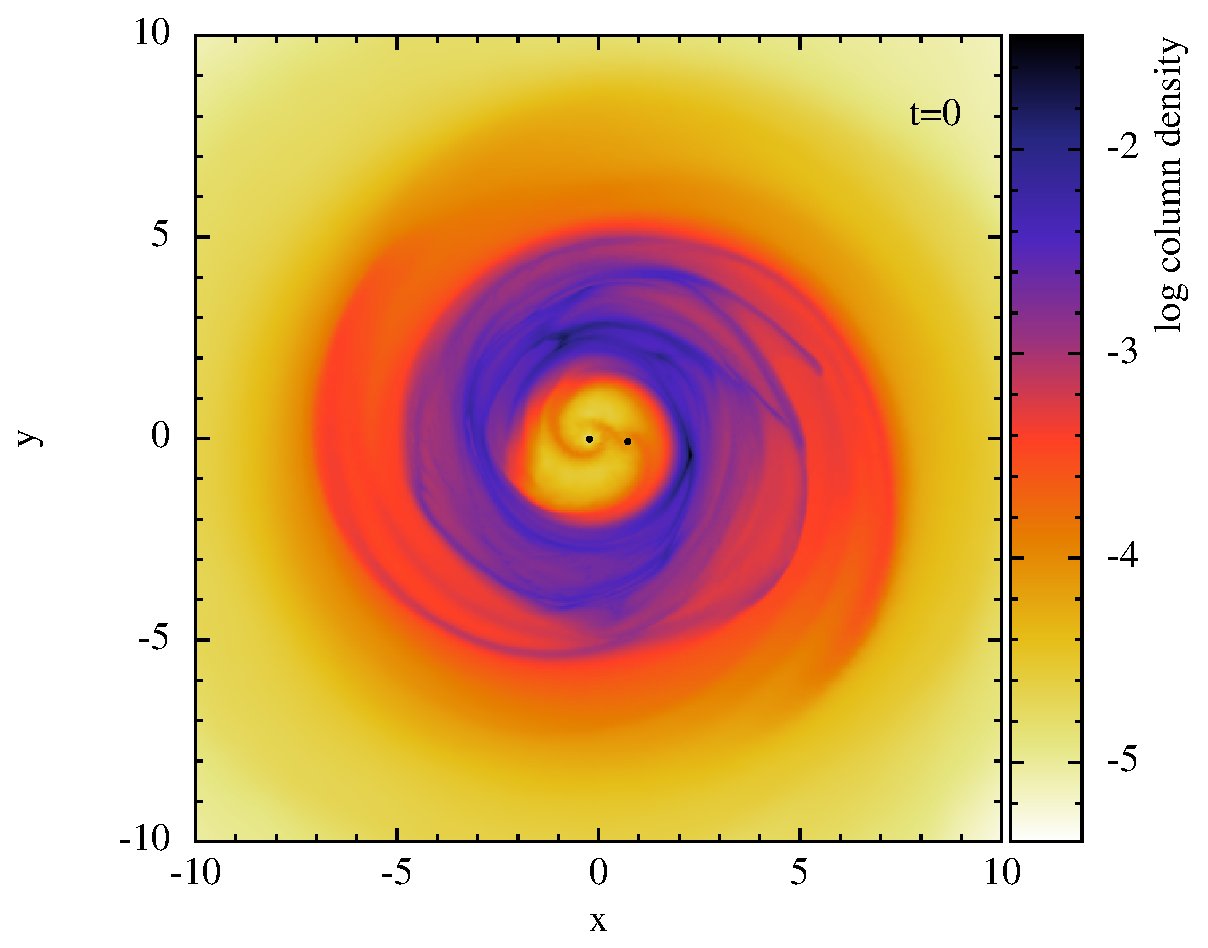
\includegraphics[width=0.45\textwidth]{figs/ic.eps}
  \caption{Left: Face-on view of the disc at $t=0$. Right: Face-on view of the disc we use to seed the magnetic fields, 
  shown as a column density map. The black dots show the position of the two SMBHs.}
 \end{center}
\end{figure}

We study three distinct domains: the cavity ($r<2$), the disc ($2<r<7, \lvert z \rvert <1$) and the outside ($r>2, \lvert z \rvert >1$) (Fig. 3).
\begin{figure}[!ht]
 \begin{center}
  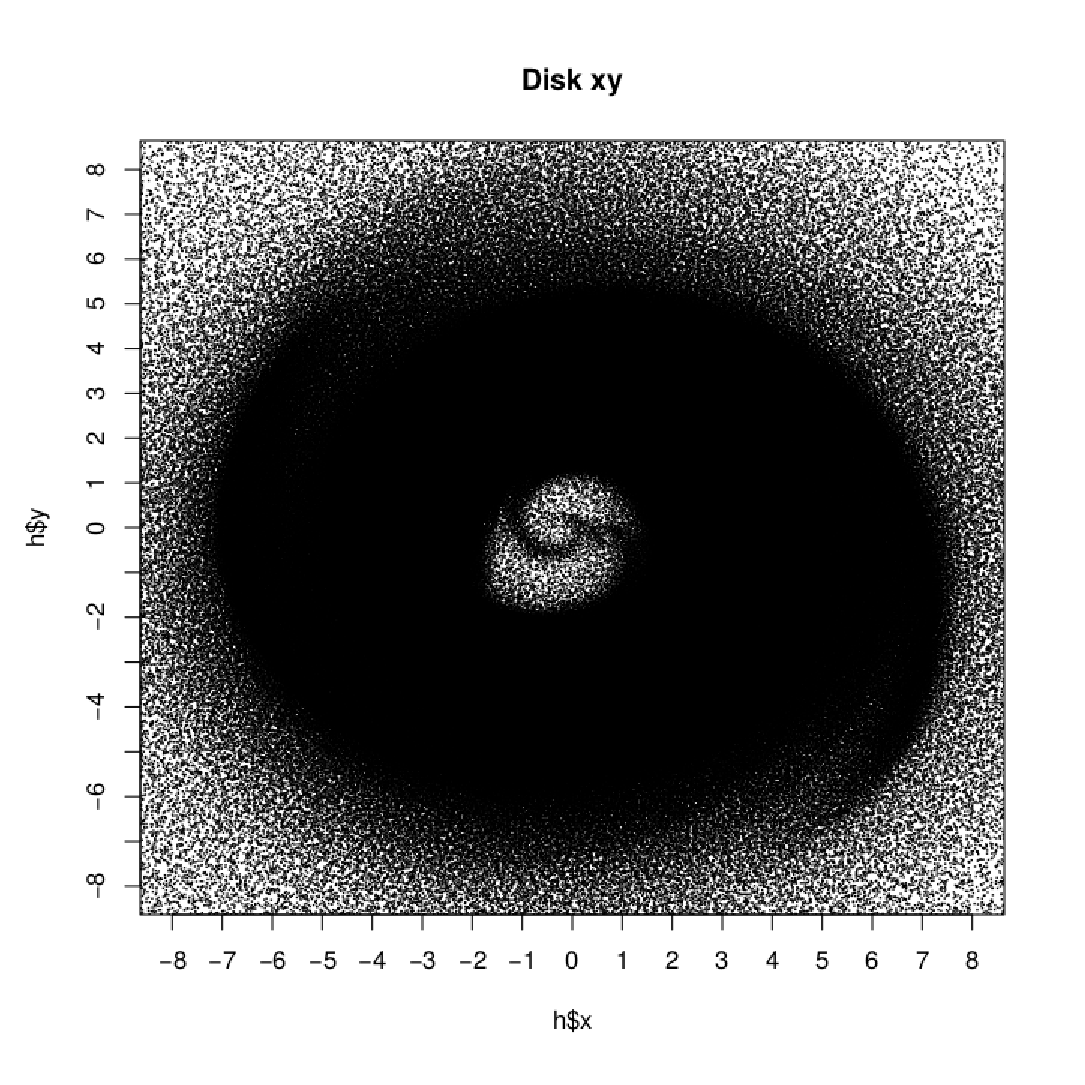
\includegraphics[width=0.4\textwidth]{figs/disk_xy.eps}
  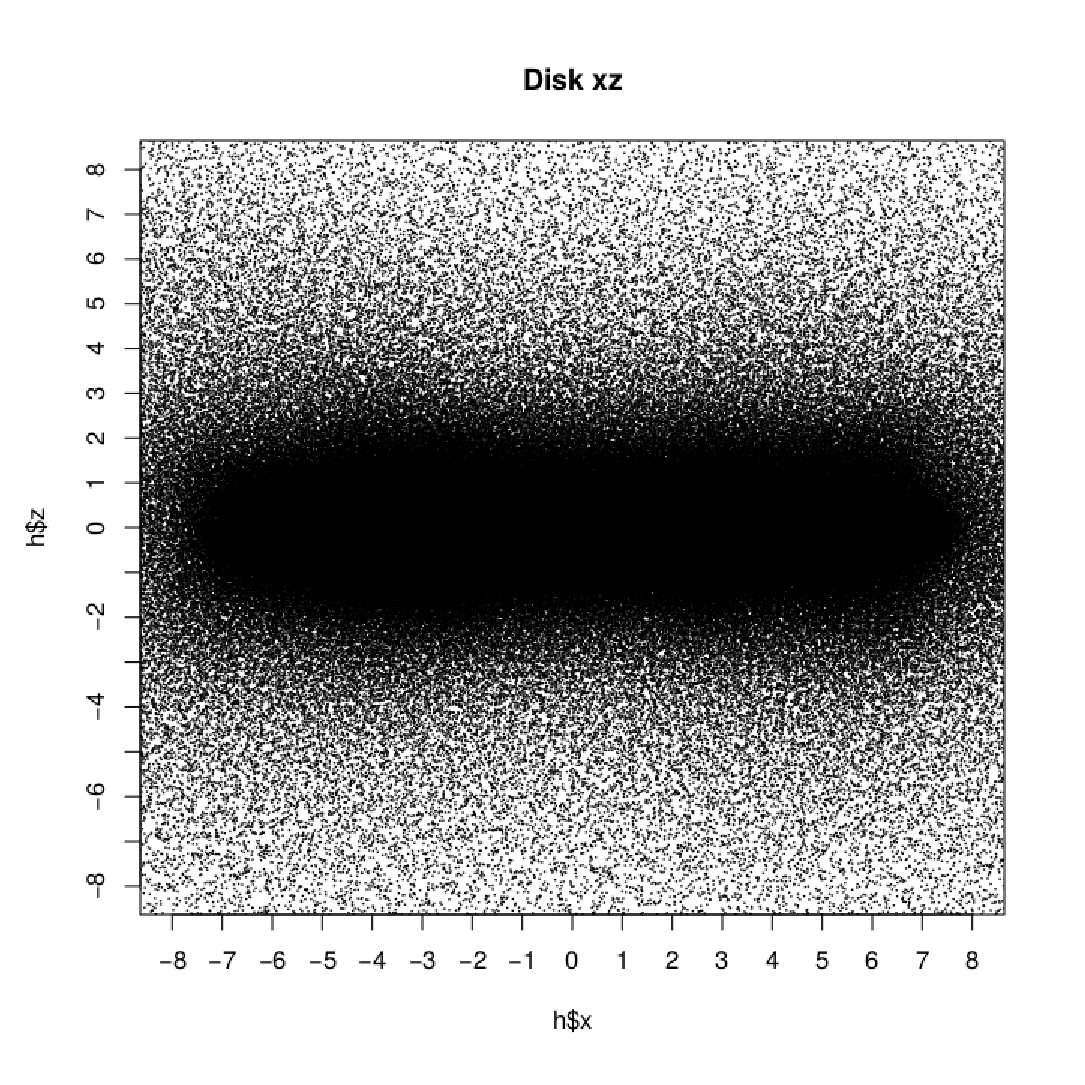
\includegraphics[width=0.4\textwidth]{figs/disk_xz.eps}
  \caption{Face-on and Edge-on views at $t=0$.}
%   cecere/R/etacs/disco.R
 \end{center}
\end{figure}

We performed a control hydrodynamical run (CON) and a run with magnetic field (MHD) until $t=350$. 
We evolved hydrodynamic (CON) and magnetohydrodynamic (MHD) adimensional equations with Gadget.
The dimensionalization is given by $l_0 = 1.2\ 10^{17}\,\text{cm}=3.9\,\text{pc}$, $m_0=6.97 \ 10^{39}\,\text{g}=3.5\ 10^6\,\text{M}_{\odot}$, 
$v_0=6.23\ 10^7\,\text{cm/s}=623\,\text{km/s}$, $t_0=61\,\text{yr}$, $\rho_0=m_0/l_0^3=4.03\ 10^{-12}\,\text{g}/\text{cm}^3$.


\section{Dynamics}
In Figures \ref{tempkindens} and \ref{eninttot}, we compared the temporal evolution of the temperature ($T$), kinetic energy ($E_{\text{kin}}$), internal energy ($E_{\text{int}}$) and total energy 
($E_{\text{tot}}=E_{\text{kin}}+E_{\text{int}}+E_{\text{mag}}$) densities for both runs, inside and outside of the disc.
\begin{figure}[!ht]
 \begin{center}
  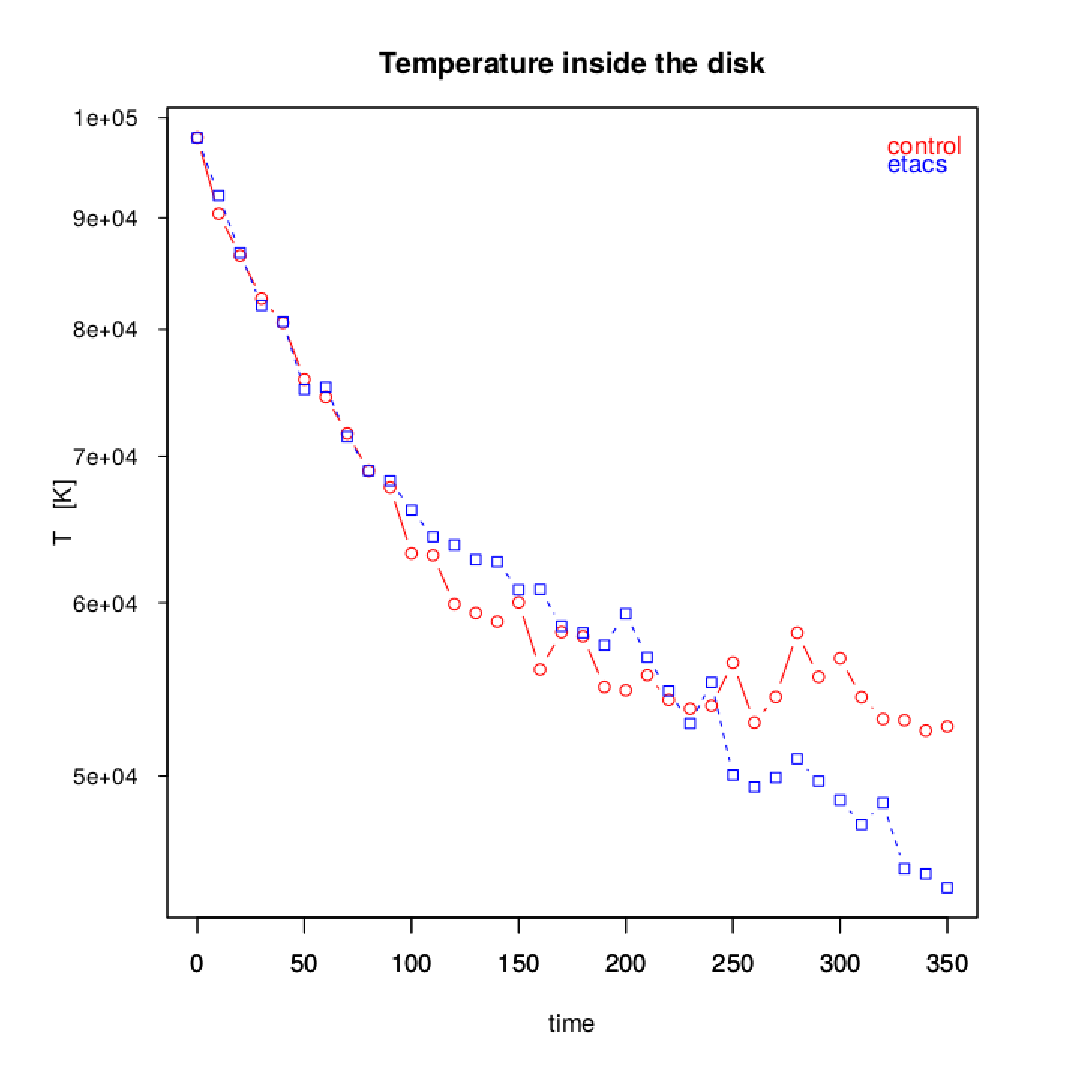
\includegraphics[width=0.45\textwidth]{figs/temp_vs_t_disco.eps}
  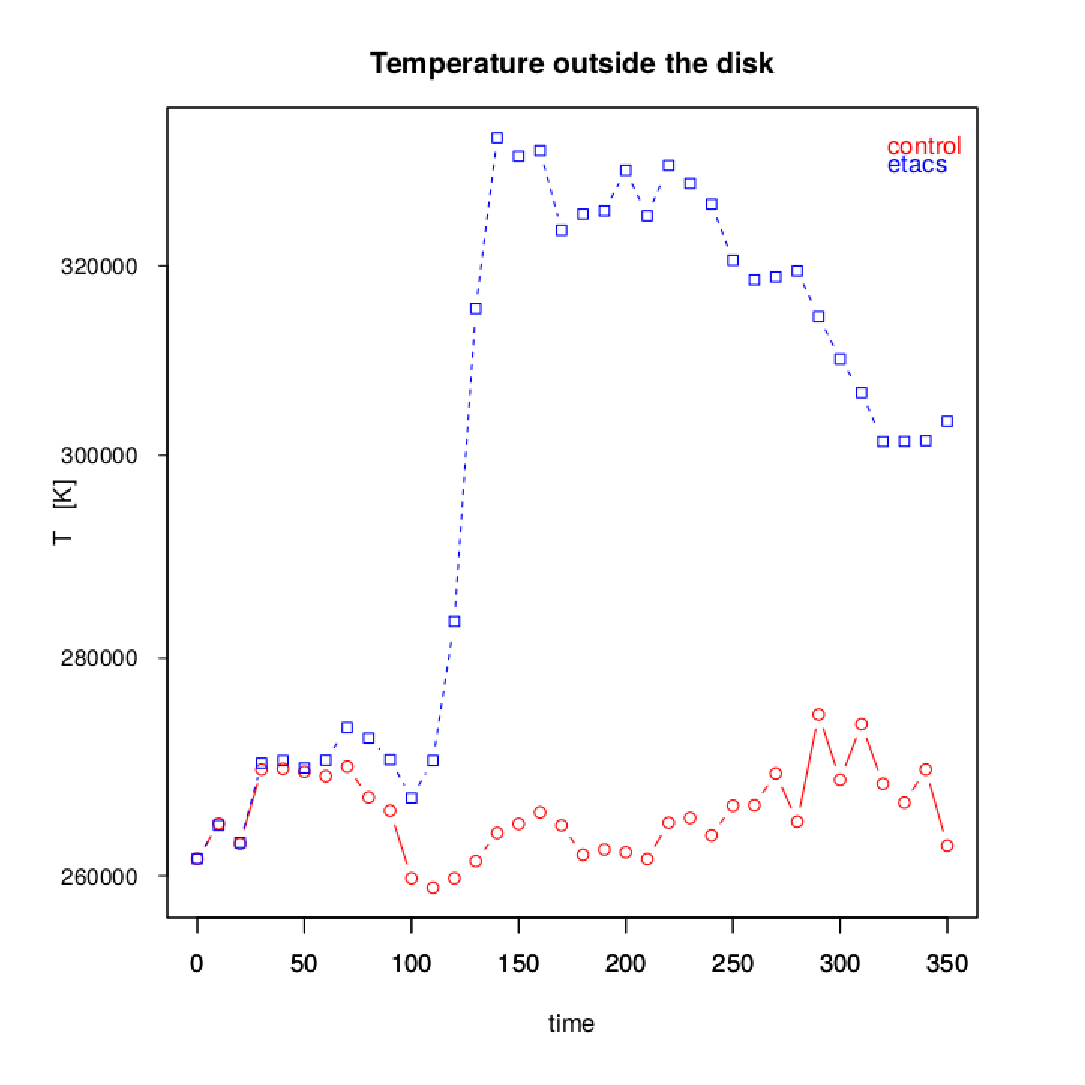
\includegraphics[width=0.45\textwidth]{figs/temp_vs_t_outside.eps}
  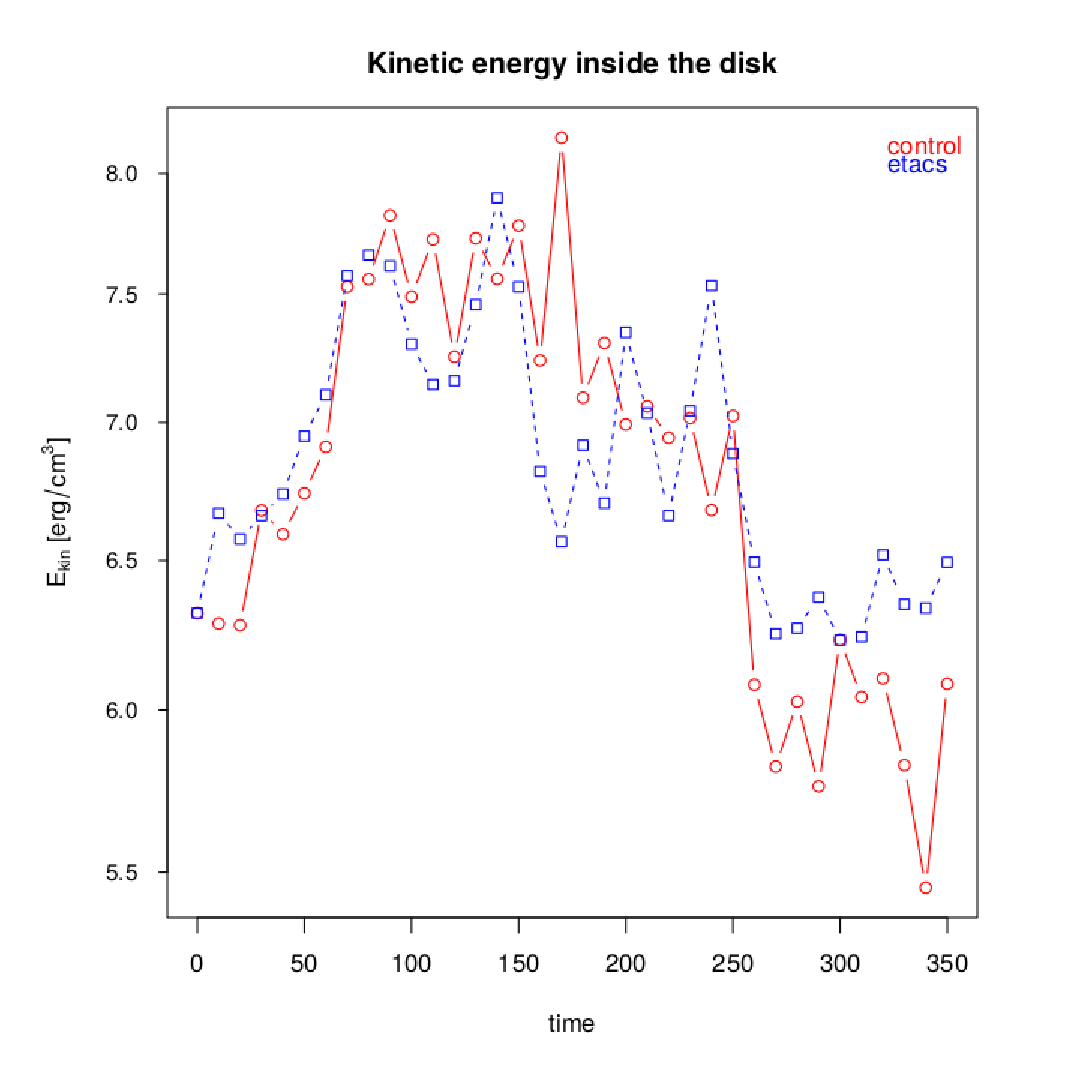
\includegraphics[width=0.45\textwidth]{figs/enkin_vs_t_disco.eps}
  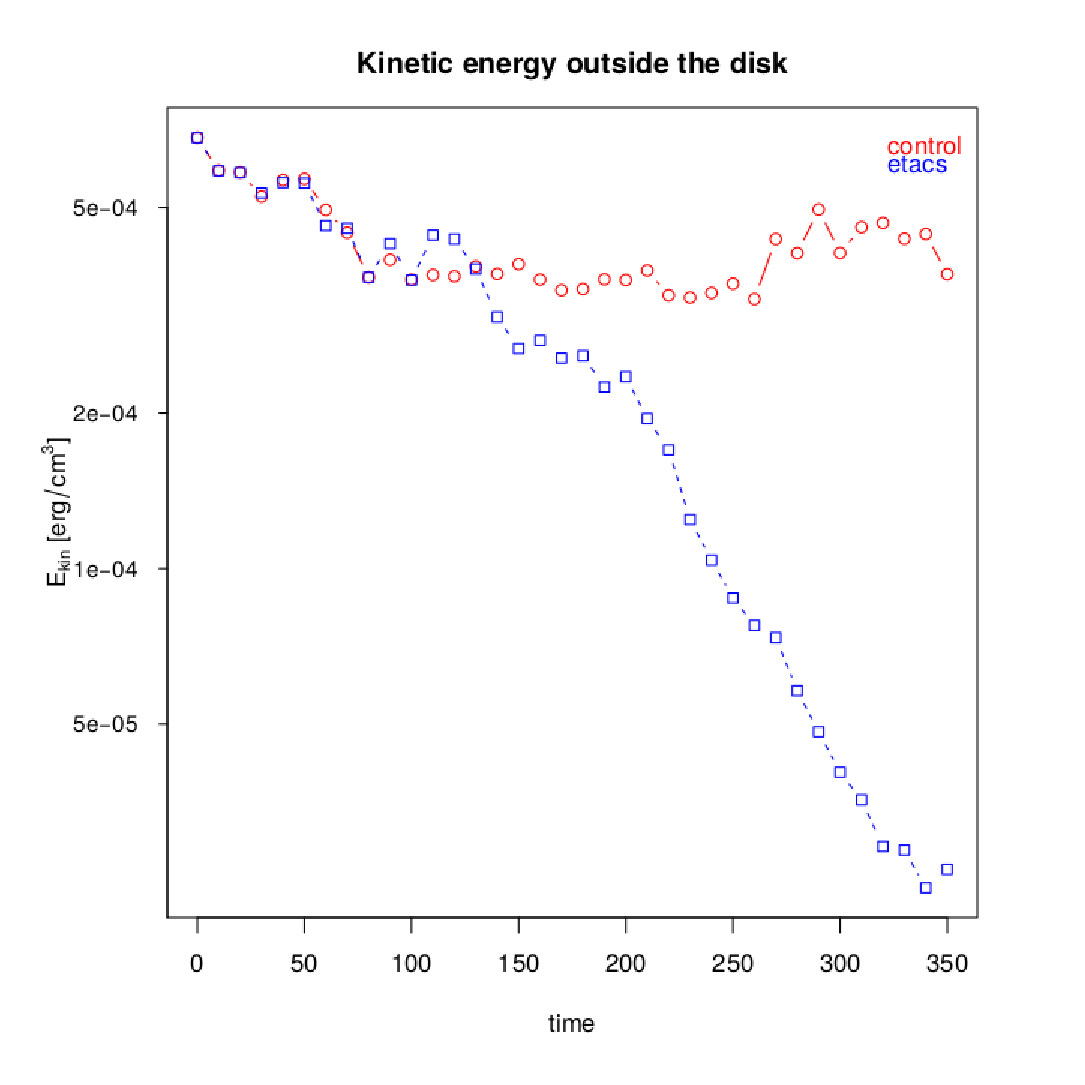
\includegraphics[width=0.45\textwidth]{figs/enkin_vs_t_outside.eps}
  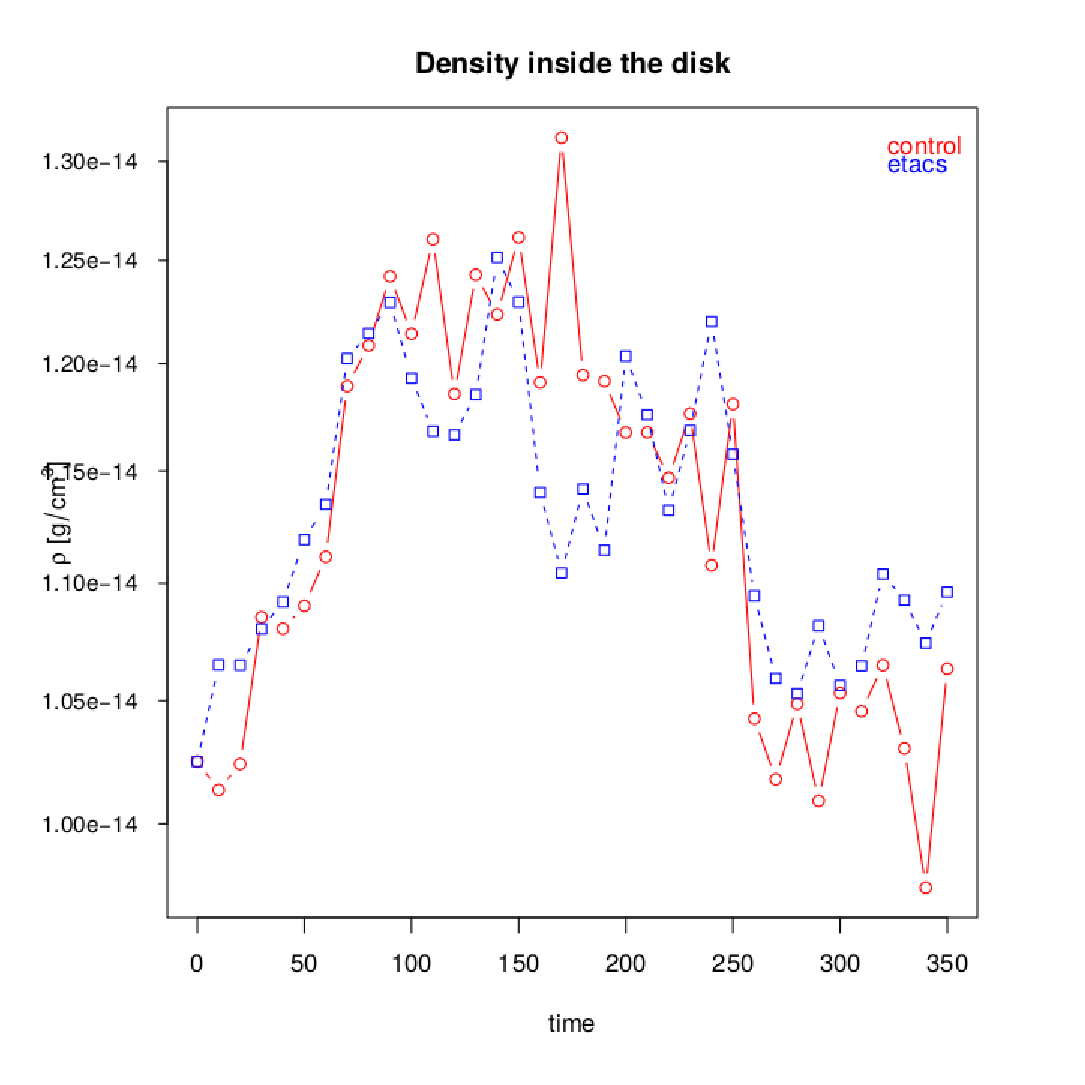
\includegraphics[width=0.45\textwidth]{figs/dens_vs_t_disco.eps}
  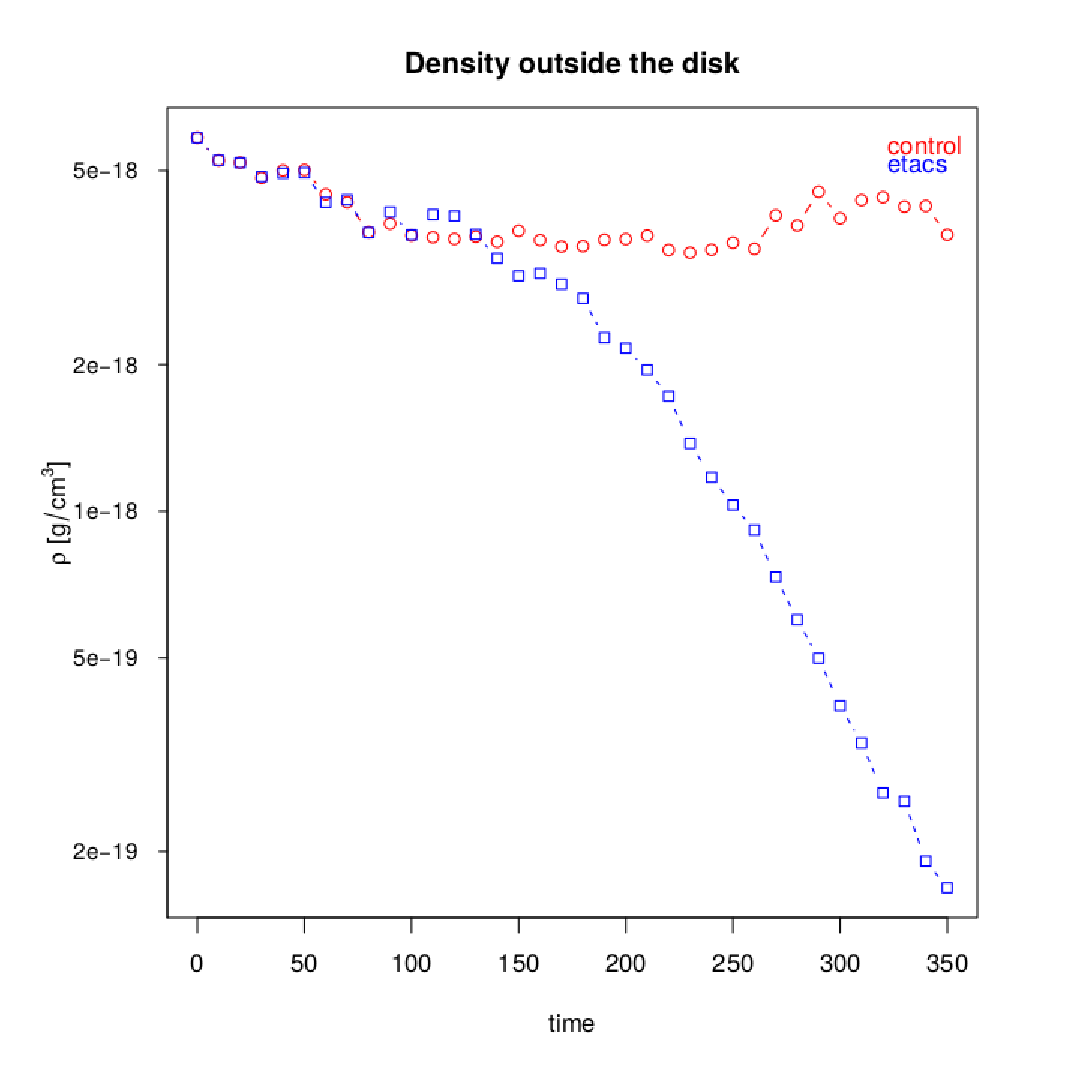
\includegraphics[width=0.45\textwidth]{figs/dens_vs_t_outside.eps}
    \caption{Temperature, kinetic energy density and number density inside and outside of the disc.}

\label{tempkindens}
 \end{center}
\end{figure}

\begin{figure}[!ht]
 \begin{center}
  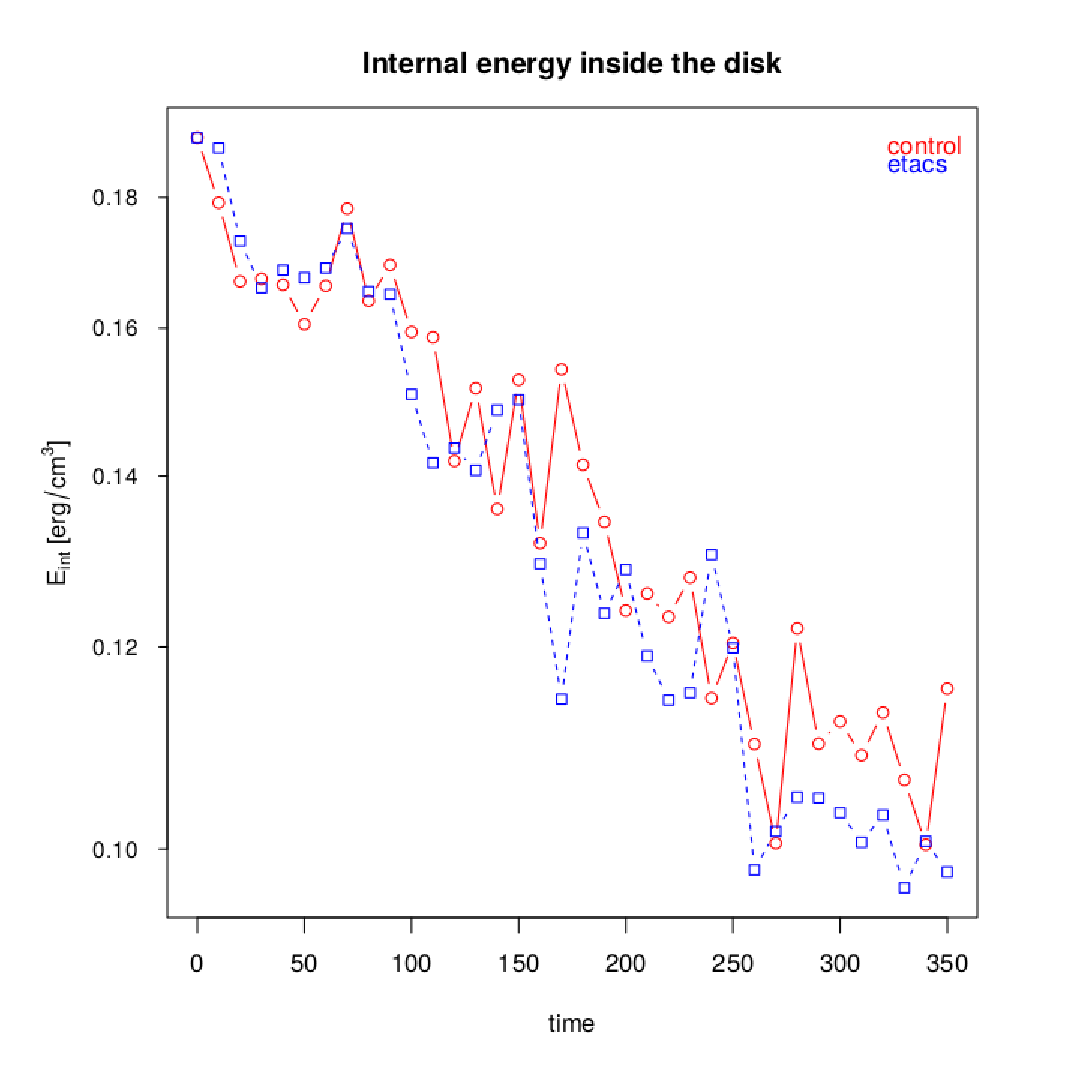
\includegraphics[width=0.45\textwidth]{figs/enint_vs_t_disco.eps}
  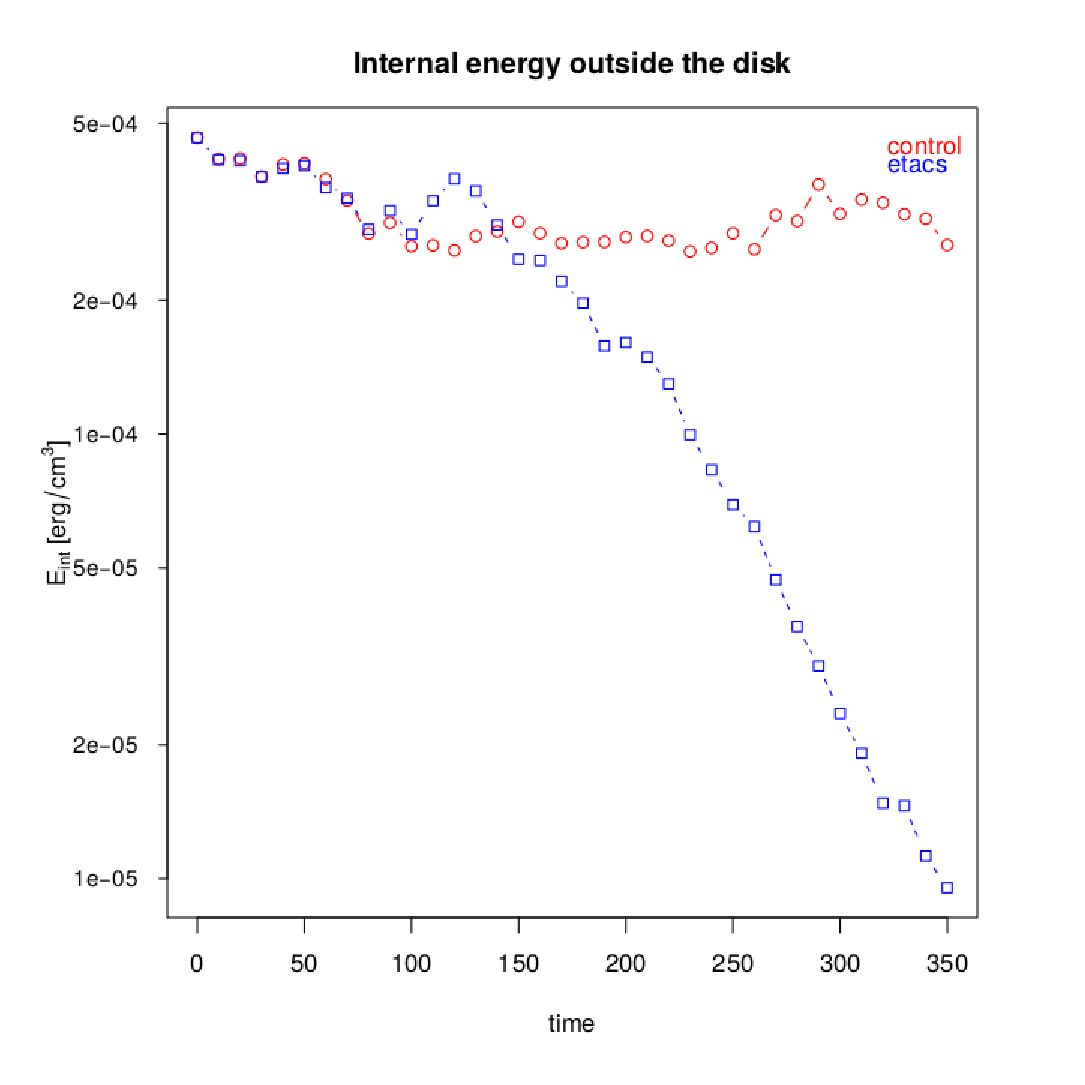
\includegraphics[width=0.45\textwidth]{figs/enint_vs_t_outside.eps}
  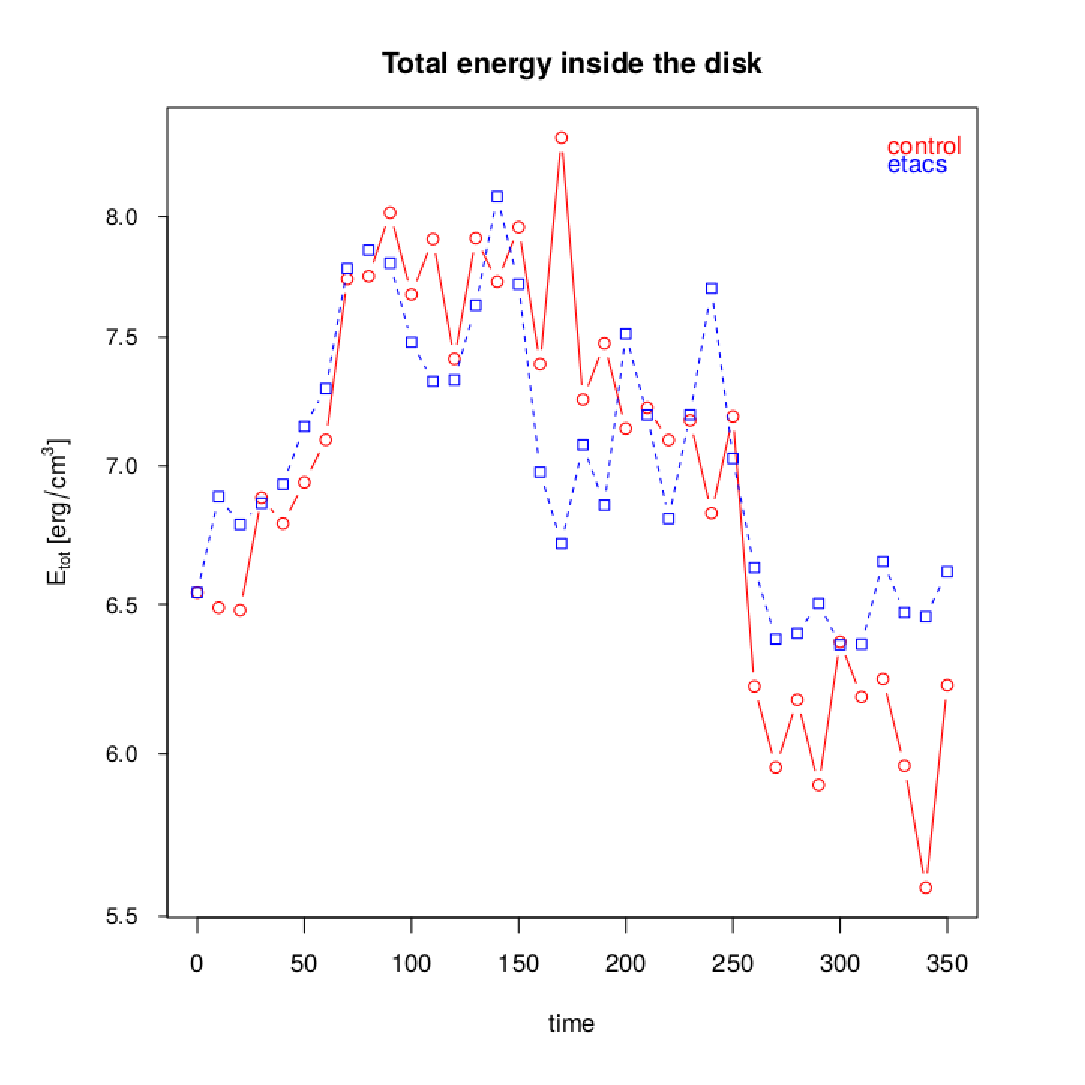
\includegraphics[width=0.45\textwidth]{figs/entot_vs_t_disco.eps}
  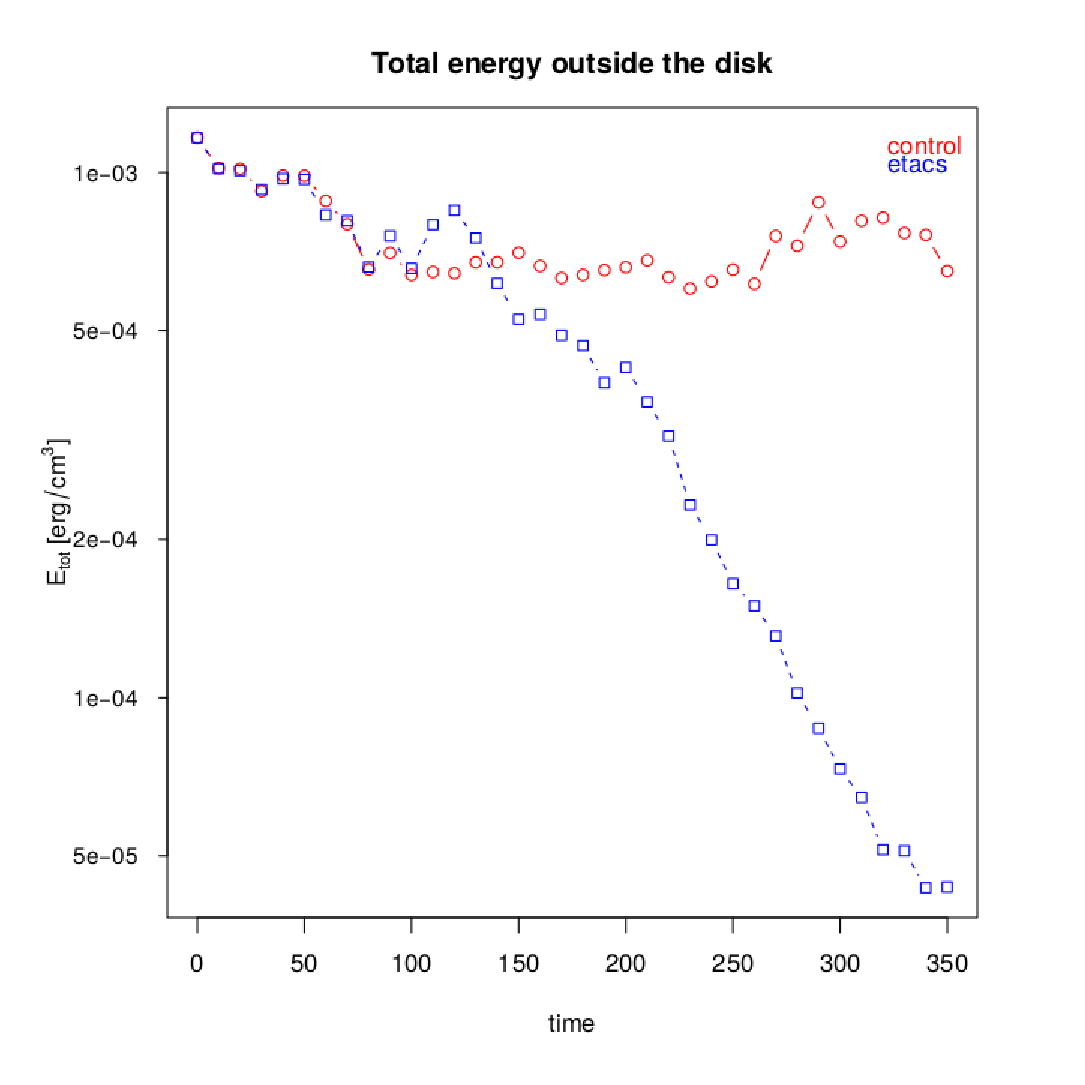
\includegraphics[width=0.45\textwidth]{figs/entot_vs_t_outside.eps}

  \caption{Internal energy and total energy density inside and outside of the disc.}

\label{eninttot}
 \end{center}
\end{figure}

We plot the magnetic energy in figure \ref{enmag} and all energy densities in figure \ref{energies},
inside and outside of the disc for MHD run.

\begin{figure}[!ht]
 \begin{center}
  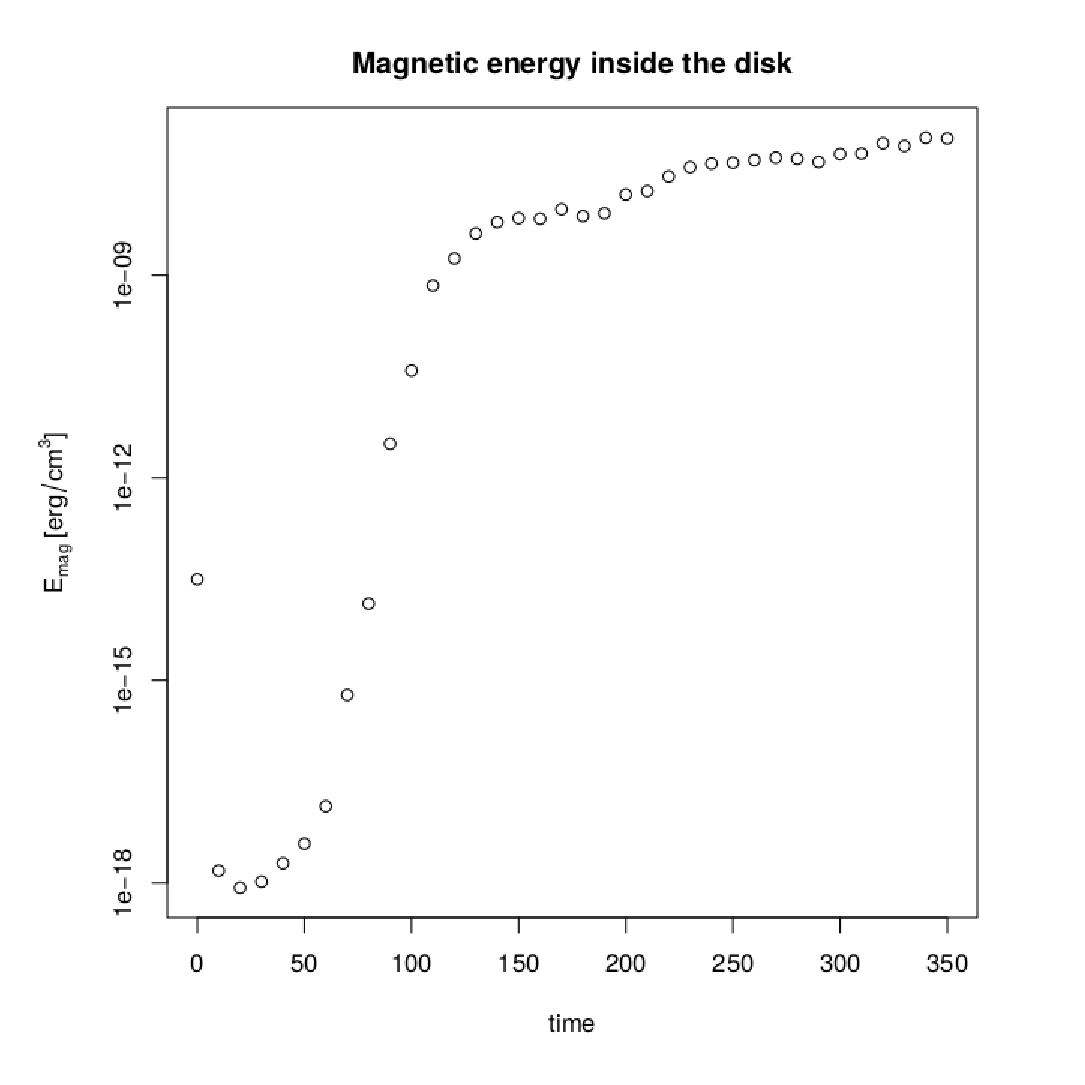
\includegraphics[width=0.45\textwidth]{figs/em_vs_t_disco.eps}
  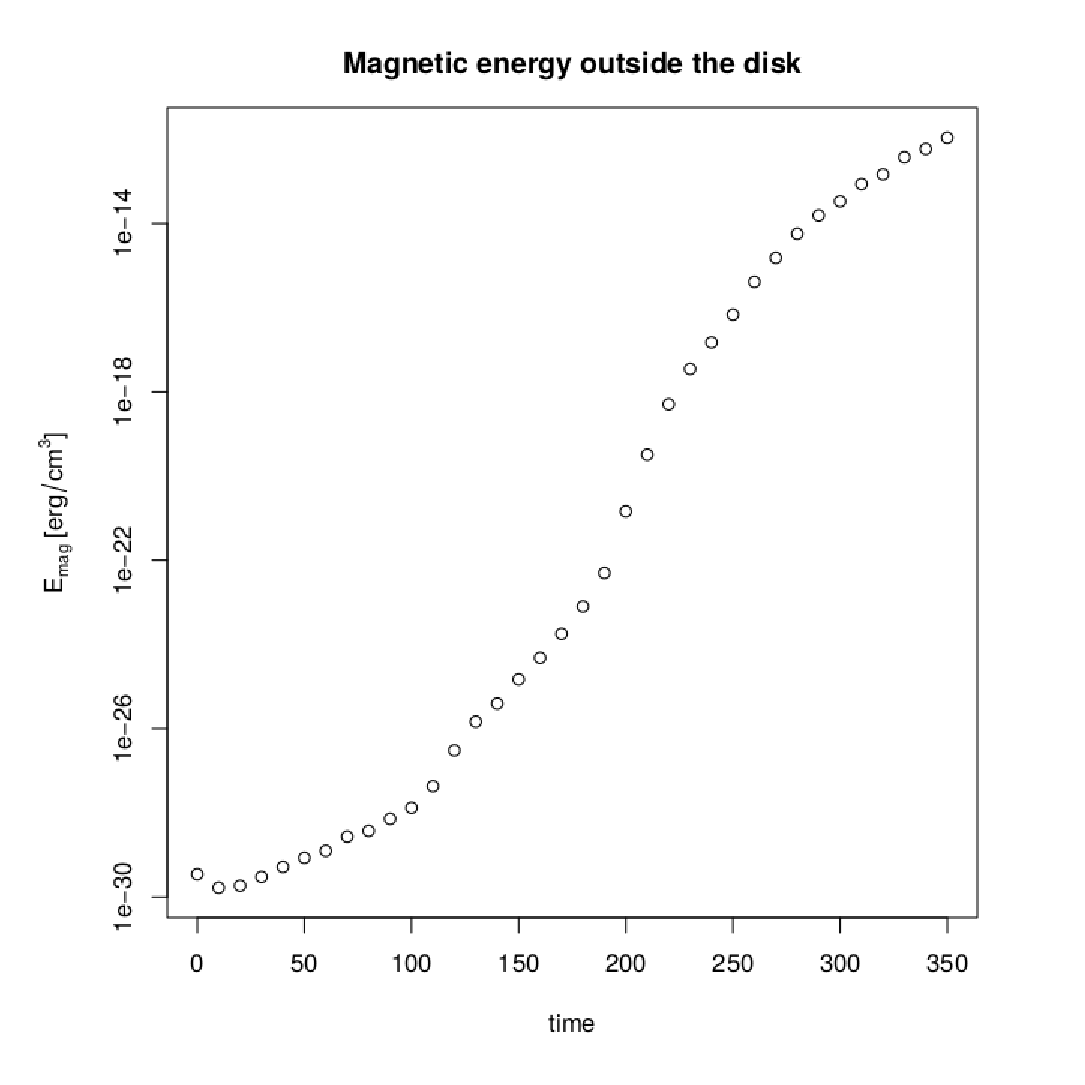
\includegraphics[width=0.45\textwidth]{figs/em_vs_t_outside.eps}
  \caption{Magnetic energy density inside and outside of the disc.}

 \label{enmag}
 \end{center}
\end{figure}

\begin{figure}[!ht]
 \begin{center}
  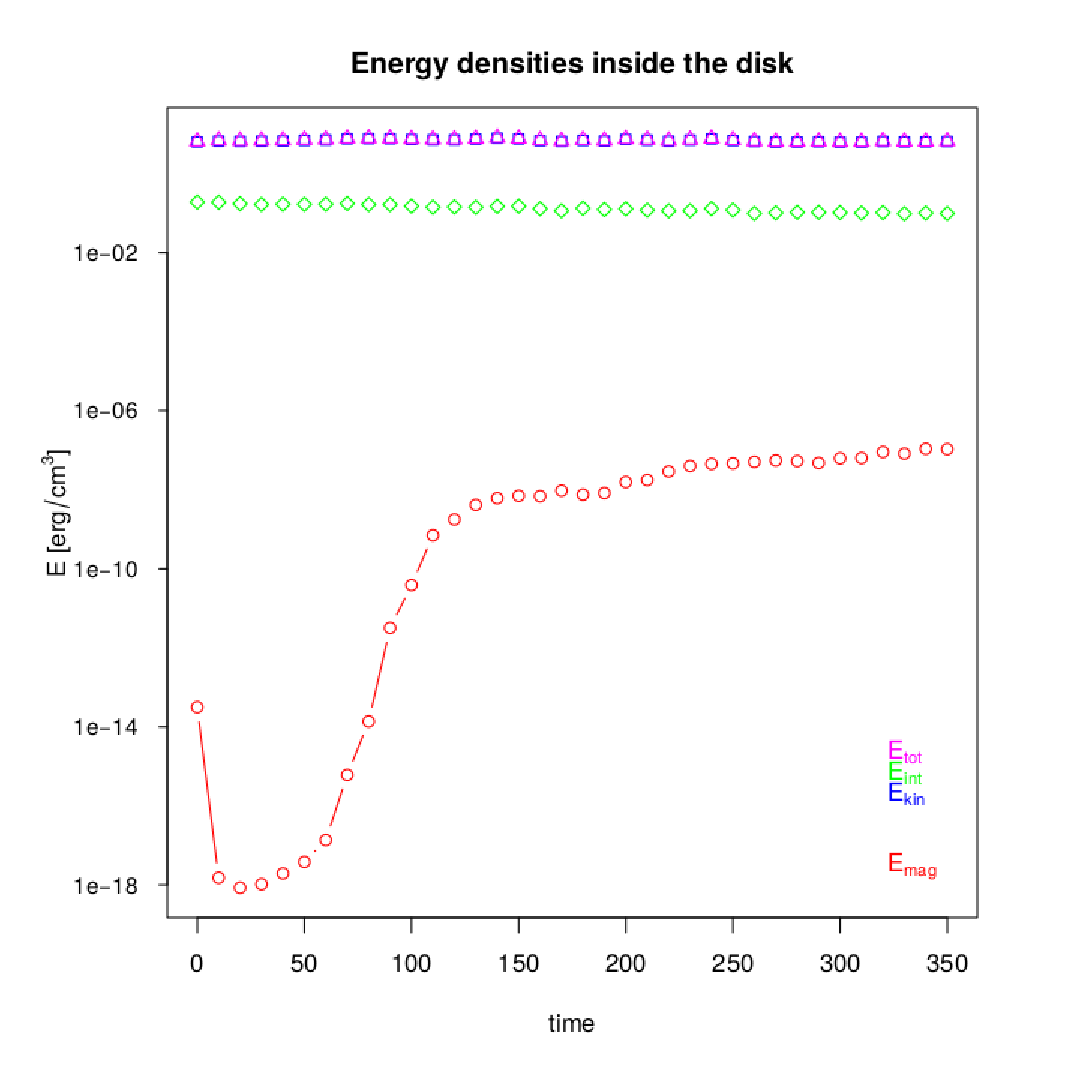
\includegraphics[width=0.45\textwidth]{figs/energies_vs_t_disco.eps}
  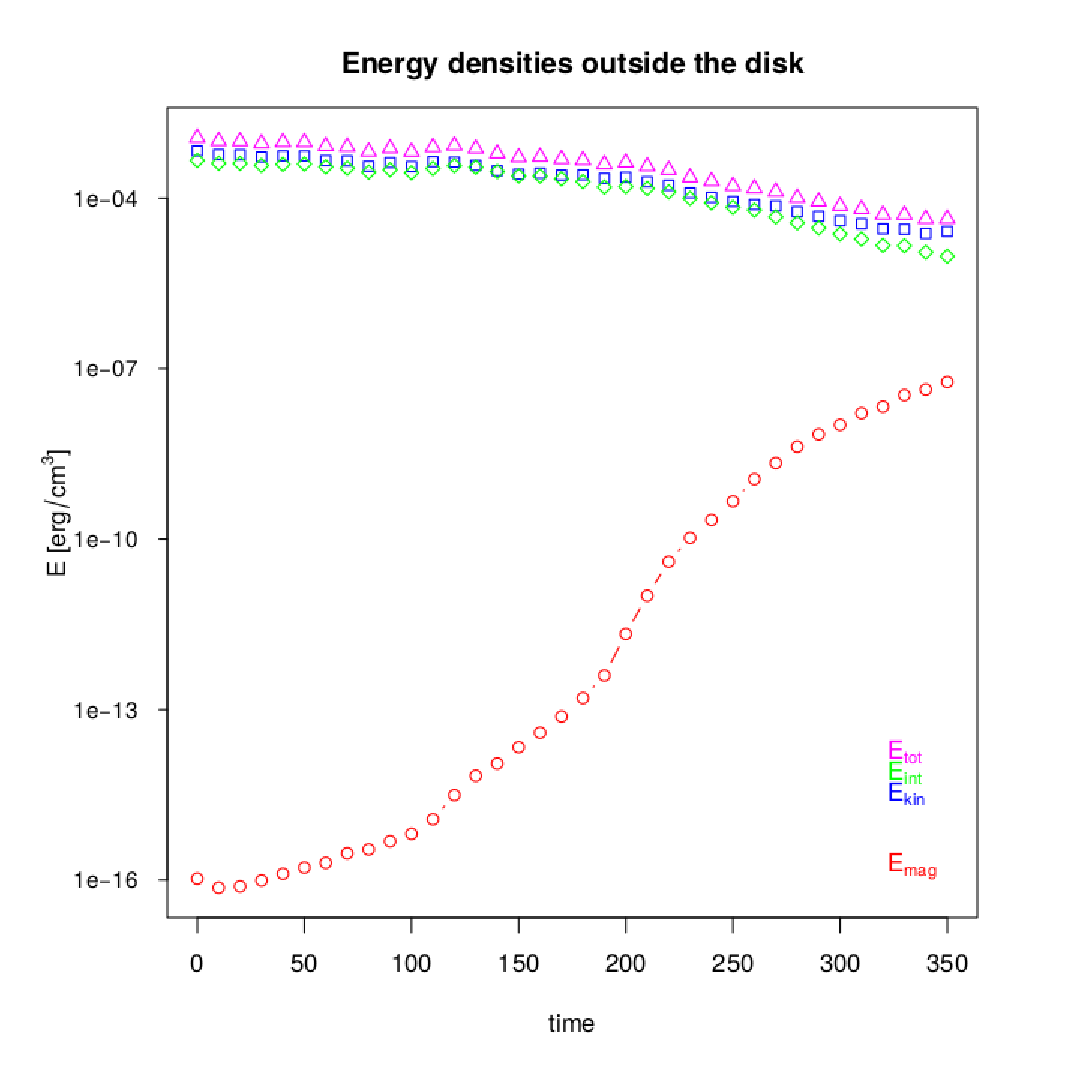
\includegraphics[width=0.45\textwidth]{figs/energies_vs_t_outside.eps}
  \caption{Energy densities inside and outside of the disc.}
%   cecere/R/etacs/disco.R
 \label{energies}
 \end{center}
\end{figure}

In Figure \ref{number} we plot the ratio between the number of particles in each zone and the initial or current total number of particles in the computational domain.
\begin{figure}[!ht]
 \begin{center}
  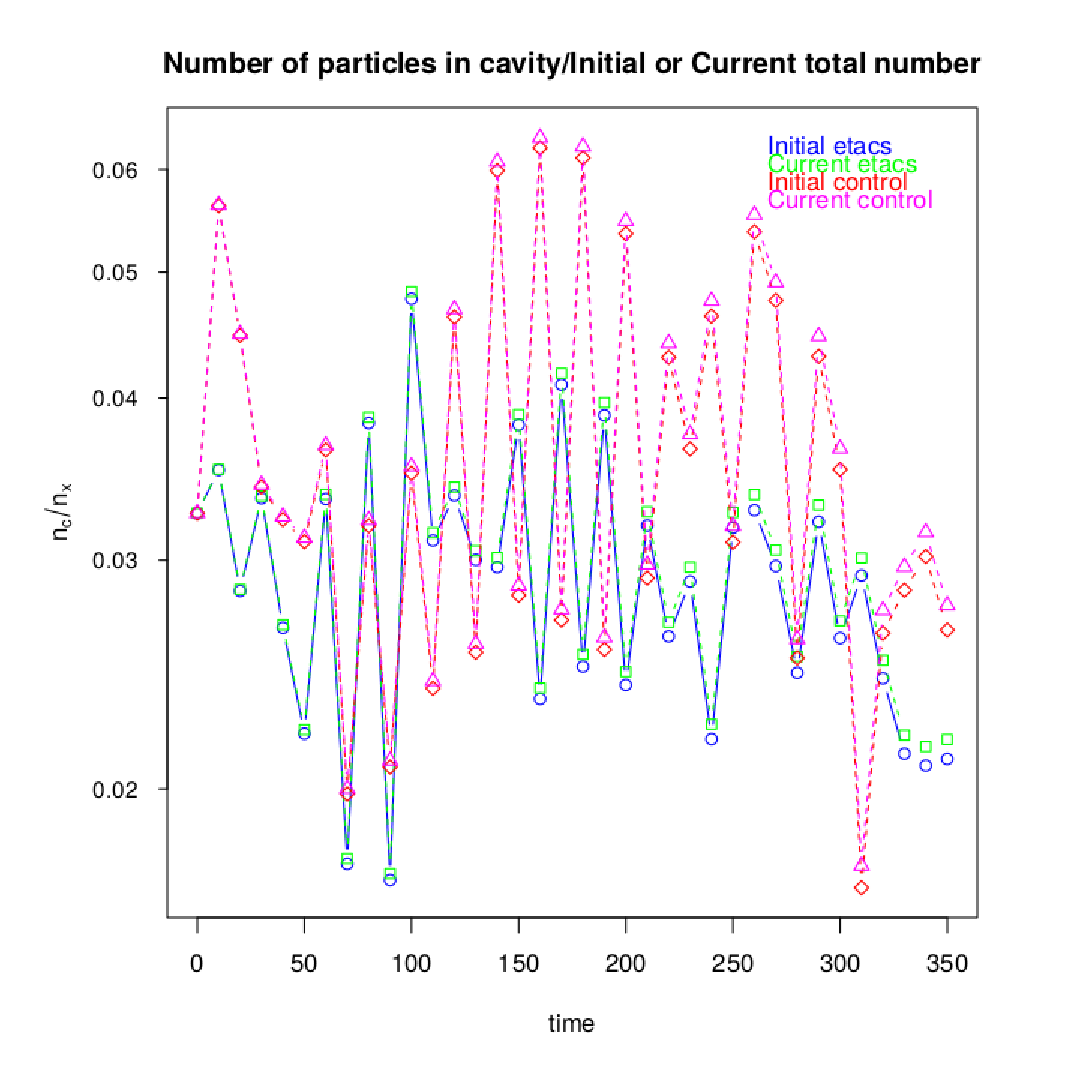
\includegraphics[width=0.3\textwidth]{figs/partnumber_vs_t_cavity.eps}
  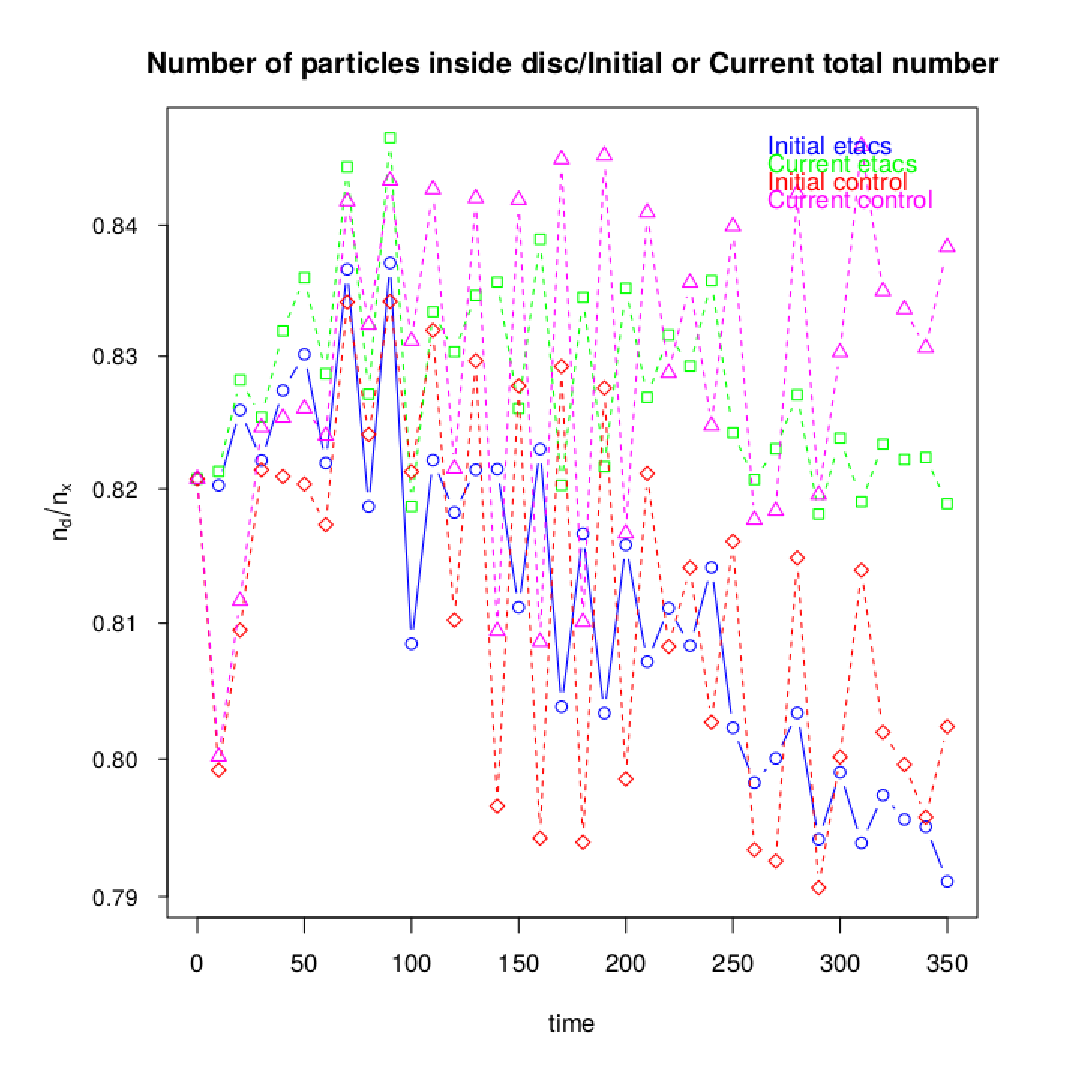
\includegraphics[width=0.3\textwidth]{figs/partnumber_vs_t_disco.eps}
  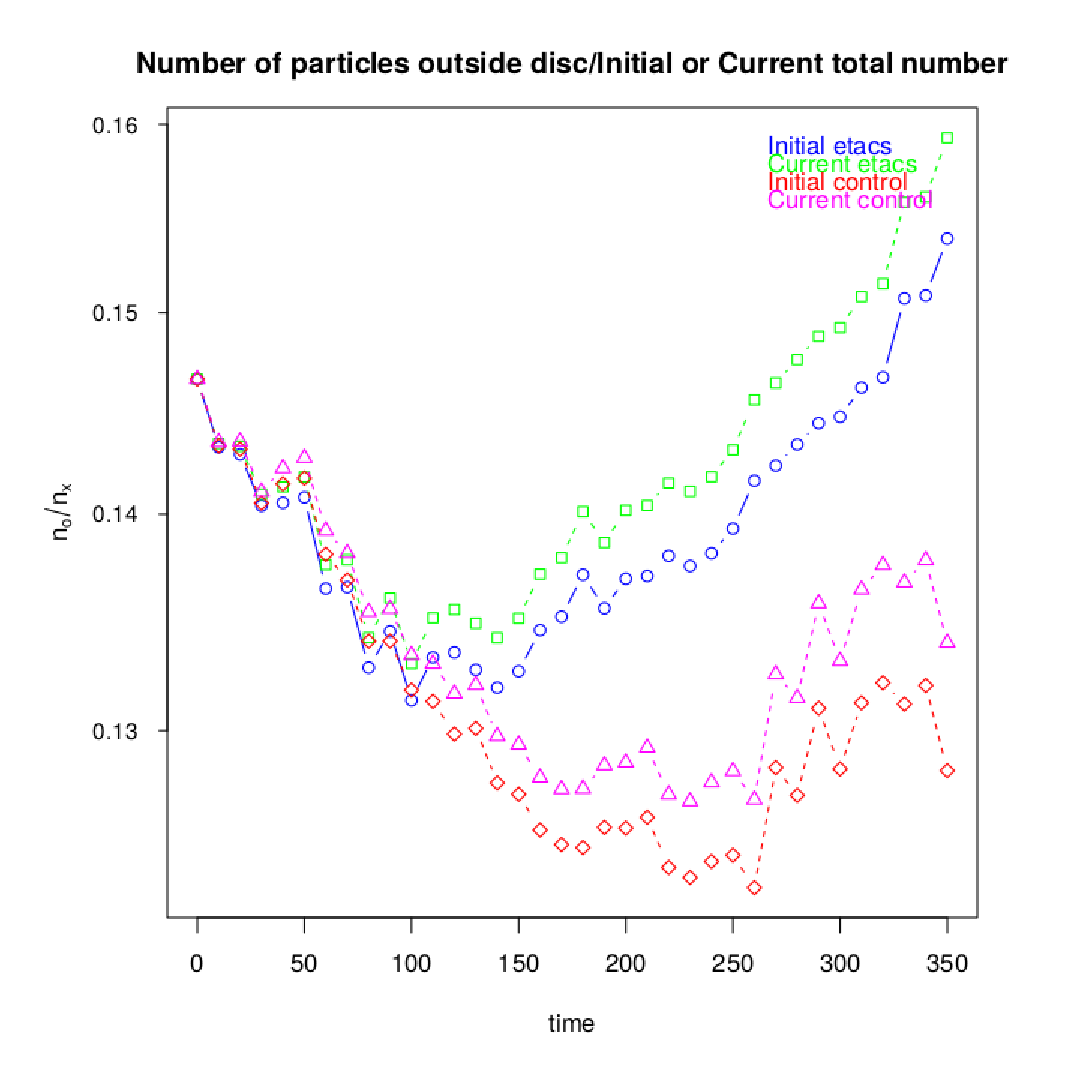
\includegraphics[width=0.3\textwidth]{figs/partnumber_vs_t_outside.eps}
  \caption{Ratio between the number of particles in cavity (left panel), inside (middle panel) and outside region (right panel) and the initial or current total number of particles
  in whole computational domain.}
%   cecere/R/etacs/disco.R
 \label{number}
 \end{center}
\end{figure}


In Figure YY we plot the evolution of the radial ($B_r$), toroidal ($B_{\phi}$) and longitudinal ($B_z$) components of the magnetic energies 
in cavity, inside disc and outside disc regions.

\begin{figure}[!ht]
 \begin{center}
  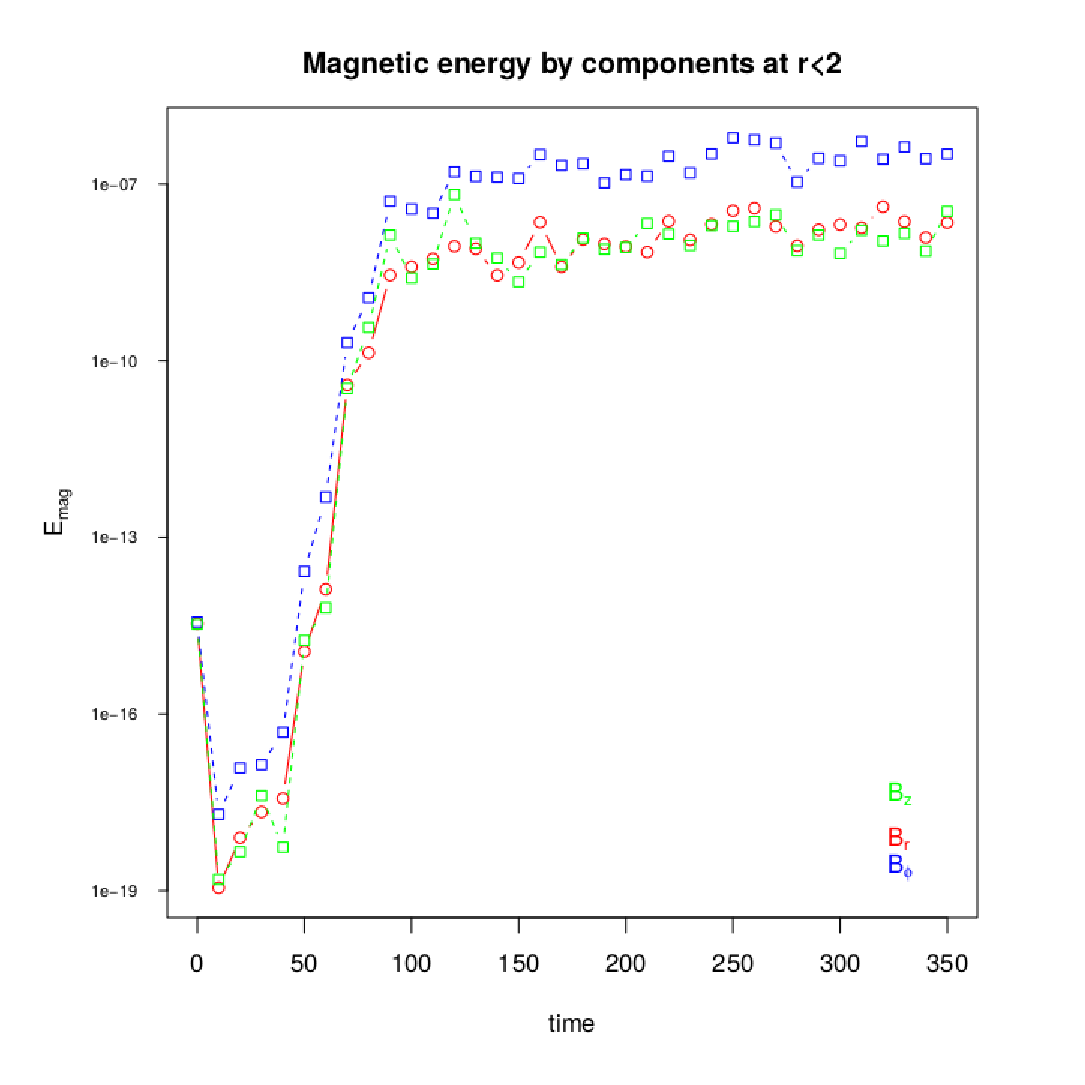
\includegraphics[width=0.3\textwidth]{figs/comp_em_vs_t_outflow.eps}
  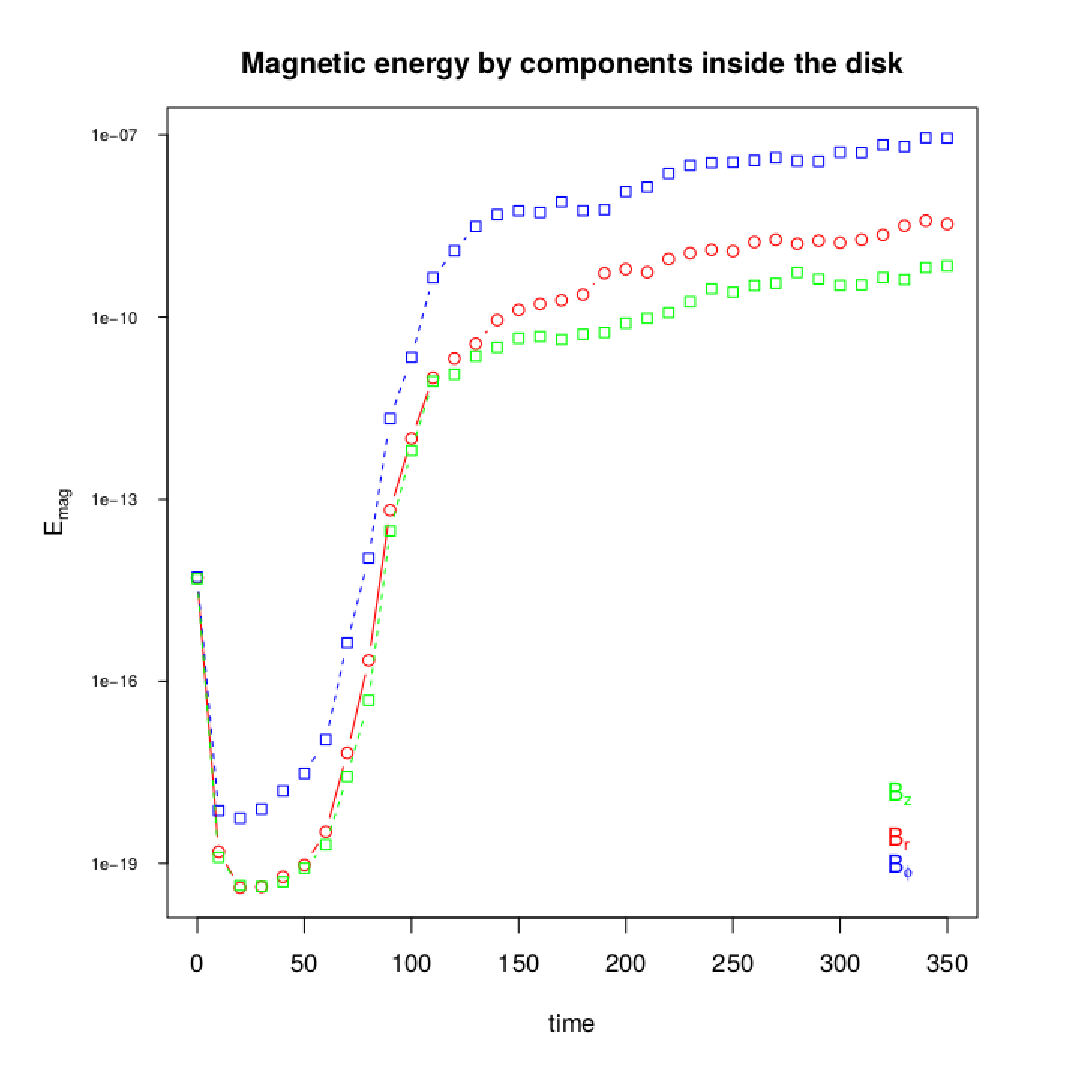
\includegraphics[width=0.3\textwidth]{figs/comp_em_vs_t_disco.eps}
  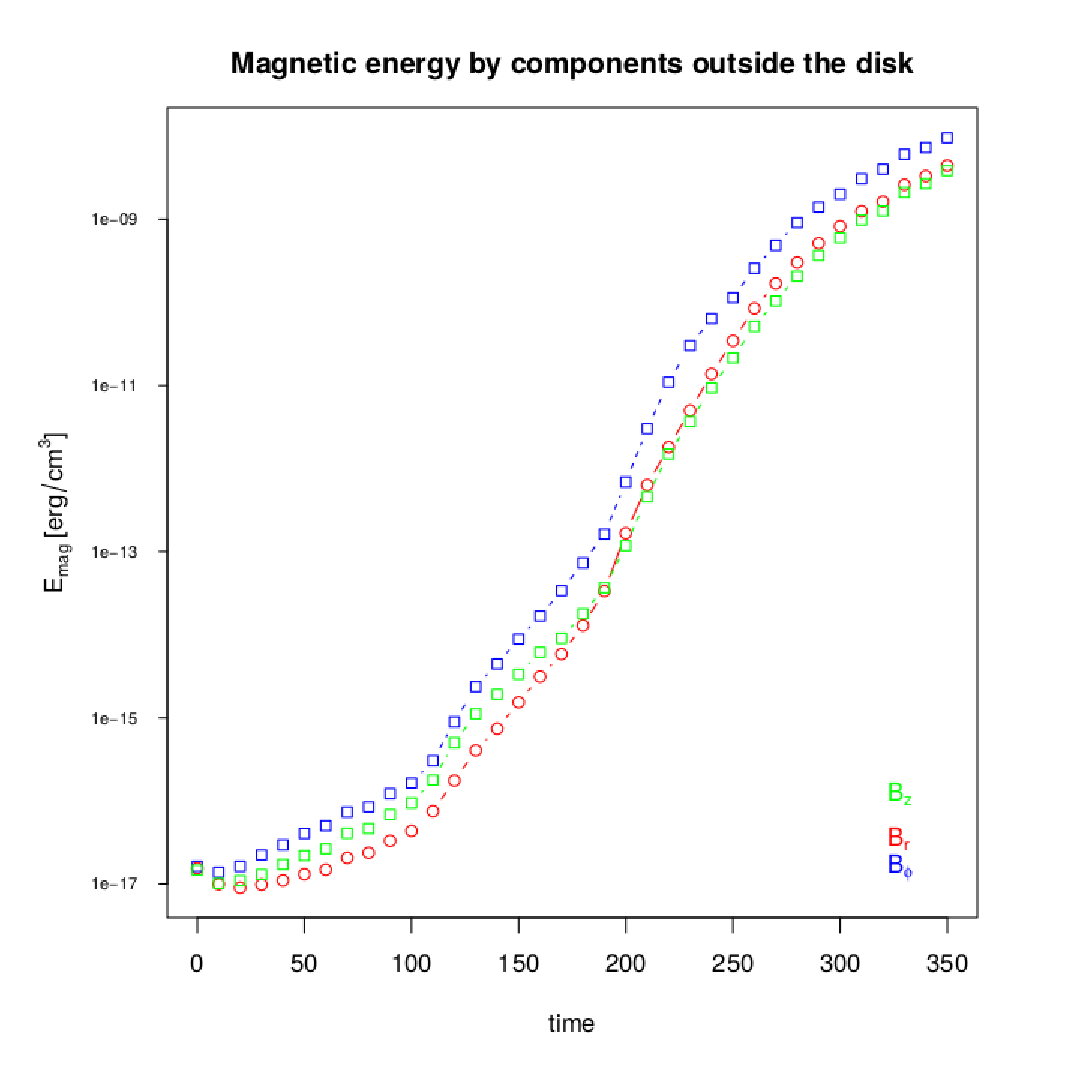
\includegraphics[width=0.3\textwidth]{figs/comp_em_vs_t_outside.eps}
  \caption{Magnetic energy by components in the cavity (left panel), inside disc (middle panel) and outside disc (right panel) regions.}
%   cecere/R/etacs/disco.R
 \label{energies}
 \end{center}
\end{figure}

\section{Clumps}

In this section we analyzed the behaviour of the clumps.

\end{document}


